\documentclass[10pt,a4paper,oneside]{article}
\usepackage[utf8]{inputenc}
\usepackage[T1]{fontenc}
\usepackage{newpxtext}
\usepackage[scaled=0.88]{sourcecodepro}
\usepackage{microtype}
\usepackage[a4paper,top=19mm,bottom=19mm,left=20mm,right=20mm,headheight=16pt,footskip=10mm]{geometry}
\usepackage[dvipsnames,table]{xcolor}
\usepackage{amssymb}
\usepackage{graphicx}
\usepackage{booktabs,tabularx,array}
\usepackage{enumitem}
\usepackage{listings}
\usepackage{tikz}
\usetikzlibrary{arrows.meta,positioning}
\usepackage{titlesec}
\usepackage{fancyhdr}
\usepackage{hyperref}
\definecolor{politoNavy}{RGB}{0,45,98}
\definecolor{steelBlue}{RGB}{35,100,160}
\definecolor{skyBlue}{RGB}{230,240,250}
\definecolor{bodyGray}{RGB}{80,85,90}
\definecolor{codeBg}{RGB}{248,249,251}
\definecolor{codeFrame}{RGB}{220,225,230}
\hypersetup{colorlinks=true,linkcolor=politoNavy,urlcolor=steelBlue,pdftitle={Laboratory 04 complete solution},pdfauthor={Politecnico di Torino}}
\titleformat{\section}{\normalfont\sffamily\Large\bfseries\color{politoNavy}}{\thesection}{0.8em}{}
\titleformat{\subsection}{\normalfont\sffamily\large\bfseries\color{steelBlue}}{\thesubsection}{0.8em}{}
\pagestyle{fancy}\fancyhf{}
\fancyhead[L]{\small\sffamily\color{bodyGray}\nouppercase{\rightmark}}
\fancyhead[R]{\small\sffamily\bfseries\thepage}
\renewcommand{\headrulewidth}{0.4pt}
\fancypagestyle{plain}{\fancyhf{}\fancyfoot[C]{\small\sffamily\thepage}\renewcommand{\headrulewidth}{0pt}}
\lstdefinestyle{studycode}{
  language=Python,basicstyle=\fontsize{7.4}{8.8}\ttfamily,
  keywordstyle=\bfseries\color{politoNavy},commentstyle=\itshape\color{bodyGray},
  stringstyle=\color{ForestGreen},numbers=left,numberstyle=\tiny\color{bodyGray},
  numbersep=6pt,tabsize=4,showstringspaces=false,breaklines=true,
  breakatwhitespace=false,columns=fullflexible,keepspaces=true,
  frame=single,rulecolor=\color{codeFrame},backgroundcolor=\color{codeBg},
  literate={█}{{\ensuremath{\blacksquare}}}1 {▎}{{|}}1 {▋}{{|}}1 {—}{{---}}1 {’}{{'}}1
}
\lstdefinestyle{terminalOutput}{
  basicstyle=\fontsize{7.2}{8.5}\ttfamily,breaklines=true,breakatwhitespace=false,
  columns=fullflexible,keepspaces=true,showstringspaces=false,
  frame=single,rulecolor=\color{codeFrame},backgroundcolor=\color{codeBg},
  literate={█}{{\ensuremath{\blacksquare}}}1 {▎}{{|}}1 {▋}{{|}}1 {—}{{---}}1 {’}{{'}}1
}
\lstset{style=studycode}
\setlist{nosep,leftmargin=1.5em}
\newcommand{\labSolutionTitle}{Laboratory 04: Causal Language Modeling and Instruction-Tuned LLMs}
\newcommand{\labSolutionSubtitle}{Complete notebook-aligned solution}
\begin{document}
\begin{titlepage}
\centering
\vspace*{8mm}

\includegraphics[width=0.30\textwidth]{../../figures/branding/polito_logo.pdf}\par
\vspace{8mm}
{\large\scshape Politecnico di Torino\par}
\vspace{2mm}
{\normalsize Master of Science in Computer Engineering\par}
{\small Department of Control and Computer Engineering (DAUIN)\par}
\vspace{12mm}
\rule{\linewidth}{1.2pt}\par\vspace{5mm}
{\Huge\bfseries\color{politoNavy}Large Language Models\\[2mm]for Software Engineering\par}
\vspace{6mm}
{\Large\bfseries\color{steelBlue}\labSolutionTitle\par}
\vspace{3mm}
{\large\labSolutionSubtitle\par}
\vspace{5mm}
\rule{\linewidth}{1.2pt}\par
\vfill
\begin{minipage}[t]{0.47\textwidth}
\raggedright
\emph{Course Instructor}\par
\textbf{Prof.~Flavio Giobergia}\par\vspace{5mm}
\emph{Laboratory Assistant}\par
\textbf{Claudio Savelli}
\end{minipage}\hfill
\begin{minipage}[t]{0.47\textwidth}
\raggedleft
\emph{Prepared by}\par
\textbf{Nicola Beccaceci}\par\vspace{5mm}
\emph{Academic Year}\par
\textbf{2026/2027}
\end{minipage}
\vfill
{\small\sffamily\color{bodyGray}Politecnico di Torino\quad|\quad Torino, Italy\par}
\end{titlepage}

\tableofcontents
\clearpage
\documentclass[../labs.tex]{subfiles}
egin{document}

\section{Exercise 1: GPT-2 medical-domain adaptation}

\label{sec:lab04-clm}

This exercise adapts pretrained GPT-2 to a small, reproducibly selected set of PubMed abstracts. Starting with 1,000 training and 500 evaluation examples, it follows tokenization and next-token labels through fine-tuning, checkpoint saving, and before/after generation from the same clinical-style prompt. The final extension compares fixed and dynamic padding, first by counting every example and then in matched short training runs. Along the way, we check that causal targets align after the model's internal shift, padded positions contribute no loss, and the timing settings match.

\begin{figure}[htbp]
\centering
\resizebox{\linewidth}{!}{%
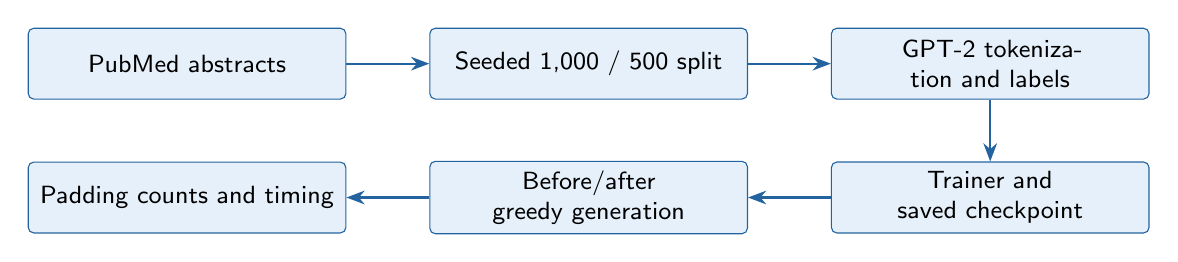
\begin{tikzpicture}[node distance=1cm, >=Stealth,
  stage/.style={draw=steelBlue,fill=skyBlue,rounded corners=2pt,
    align=center,text width=3.8cm,minimum height=0.9cm,font=\small\sffamily}]
\node[stage] (a) at (0cm,0cm) {PubMed abstracts};
\node[stage] (b) at (5.1cm,0cm) {Seeded 1,000 / 500 split};
\node[stage] (c) at (10.2cm,0cm) {GPT-2 tokenization and labels};
\node[stage] (d) at (10.2cm,-1.7cm) {Trainer and saved checkpoint};
\node[stage] (e) at (5.1cm,-1.7cm) {Before/after greedy generation};
\node[stage] (f) at (0cm,-1.7cm) {Padding counts and timing};
\draw[->,thick,steelBlue] (a) -- (b);
\draw[->,thick,steelBlue] (b) -- (c);
\draw[->,thick,steelBlue] (c) -- (d);
\draw[->,thick,steelBlue] (d) -- (e);
\draw[->,thick,steelBlue] (e) -- (f);
\end{tikzpicture}%
}
\caption{Exercise pipeline: each stage produces the state consumed by the next.}
\end{figure}

\subsection{Data, tokenization, and next-token targets}

\medskip
\noindent The notebook begins by importing the causal-language-model trainer and dataset loader, fixing the random seed, and selecting an available accelerator. This state is shared by the data preparation, model training, and the later padding experiments. The printed backend identifies the device on which the saved run was made.
\label{res:lab04-clm-0002}
% coverage-cell: LABS/lab04/text-01-clm.ipynb cell=2 source_sha256=cb8ed58a968014e96f3a117c12421bb49cf0745d7de963b4254240d0a573ef05
\begin{lstlisting}[style=studycode]
from transformers import AutoTokenizer, AutoModelForCausalLM, Trainer, TrainingArguments
from datasets import load_dataset
import torch
from transformers import set_seed

set_seed(42)
torch.set_num_threads(4)
device = "cuda" if torch.cuda.is_available() else "mps" if torch.backends.mps.is_available() else "cpu"
print(f"Training backend: {device}")
\end{lstlisting}
\par\smallskip
% coverage-output: LABS/lab04/text-01-clm.ipynb cell=2 output=0 source_sha256=cb8ed58a968014e96f3a117c12421bb49cf0745d7de963b4254240d0a573ef05 payload_sha256=bad99702ba06356362737edc9977feb1e2a443860360a023fbb64df047a2e7b2 artifact=study_guide/execution_artifacts/lab04/lab04/text-01-clm_cell_0002_cb8ed58a9680_output_0.txt
\label{out:lab04-clm-0002-00}
\textit{Complete warning/progress output is retained in the execution-artifact tree and linked to this result.}
% coverage-output: LABS/lab04/text-01-clm.ipynb cell=2 output=1 source_sha256=cb8ed58a968014e96f3a117c12421bb49cf0745d7de963b4254240d0a573ef05 payload_sha256=7922a39ef09c6b17cd84cac752c3cc3e6cde9c3a4dd8c75be1fddab679778068 artifact=study_guide/execution_artifacts/lab04/lab04/text-01-clm_cell_0002_cb8ed58a9680_output_1.txt
\label{out:lab04-clm-0002-01}
\lstinputlisting[style=terminalOutput]{../../execution_artifacts/lab04/lab04/text-01-clm_cell_0002_cb8ed58a9680_output_1.txt}
The output reports the MPS backend. This confirms that the Apple GPU path was selected for the original medical adaptation and informs how its runtime should be interpreted.

\medskip
\noindent This cell obtains the PubMed abstract collection, shuffles it with seed 42, and selects disjoint slices: indices 0--999 for training and 1,000--1,499 for evaluation. Repeating the same seeded shuffle makes the boundary reproducible. Keeping the evaluation slice separate lets the Trainer report held-out loss during fine-tuning.
\label{res:lab04-clm-0005}
% coverage-cell: LABS/lab04/text-01-clm.ipynb cell=5 source_sha256=c9928d2abedc802588a6b9046c655788a1620c7f267ce1b5fdcd195e07aa3dad
\begin{lstlisting}[style=studycode]
ds = load_dataset("japhba/pubmed_simple", split="train")
train_dataset = ds.shuffle(seed=42).select(range(1000))
eval_dataset = ds.shuffle(seed=42).select(range(1000, 1500))
\end{lstlisting}
\par\smallskip The cell creates the 1,000-example training set and 500-example evaluation set consumed by the tokenizer and Trainer.

\medskip
\noindent This inspection checks the first training record before preprocessing. It makes the actual input field and the medical-abstract content visible, so the following tokenizer can be applied to the expected text column.
\label{res:lab04-clm-0007}
% coverage-cell: LABS/lab04/text-01-clm.ipynb cell=7 source_sha256=7078f6ee92efc42b3e50a03bcfb2ba6af316950a8b621b510c4efdc8186793ff
\begin{lstlisting}[style=studycode]
train_dataset[0]
\end{lstlisting}
\par\smallskip
% coverage-output: LABS/lab04/text-01-clm.ipynb cell=7 output=0 source_sha256=7078f6ee92efc42b3e50a03bcfb2ba6af316950a8b621b510c4efdc8186793ff payload_sha256=008f47ad17beb0469d652456ec6cad79ff6122b962576ffa2ca5494068696415 artifact=study_guide/execution_artifacts/lab04/lab04/text-01-clm_cell_0007_7078f6ee92ef_output_0.txt
\label{out:lab04-clm-0007-00}
\lstinputlisting[style=terminalOutput]{../../execution_artifacts/lab04/lab04/text-01-clm_cell_0007_7078f6ee92ef_output_0.txt}
The printed dictionary contains an abstract about segmentation of abdominal images and class imbalance. It confirms that the dataset supplies the \texttt{abstract} field used in the next computation.

\medskip
\noindent This cell turns each abstract into GPT-2 token IDs. The EOS token is reused as the tokenizer's padding ID because GPT-2 has no dedicated pad token. Truncation and fixed padding produce 1,024 positions per example; the attention mask distinguishes real tokens from positions filled with that reused ID. Mapping is batched for efficiency, and the original text columns are removed after tokenization.
\label{res:lab04-clm-0010}
% coverage-cell: LABS/lab04/text-01-clm.ipynb cell=10 source_sha256=ff1882d3ed4da13a310091ce599f95615b7b09fff126ab994fddf3b610f8d158
\begin{lstlisting}[style=studycode]
# TODO: Tokenize the Dataset using the GPT-2 tokenizer
# Hint: Use the `map` method of the dataset object
model_name = "gpt2"
tokenizer = AutoTokenizer.from_pretrained(model_name)
tokenizer.pad_token = tokenizer.eos_token  # Set padding token to EOS token

def tokenize_function(samples):
    # Tokenize the text column `abstract` in the dataset (set `truncation=True` and `padding="max_length"`)
    # NOTE: You can either use tokenzier as a global variable, or
    # use a closure to capture the tokenizer variable
    return tokenizer(samples["abstract"], truncation=True, padding="max_length", max_length=1024)

# NOTE: you should map the dataset using the tokenize function. 
# (You can optionally consider using the argument `batched=True` for better performance,
# as long as tokenize_function can handle the batch! [note2: the tokenizer can do that!])
tokenized_dataset = train_dataset.map(tokenize_function, batched=True, remove_columns=train_dataset.column_names)
tokenized_dataset_eval = eval_dataset.map(tokenize_function, batched=True, remove_columns=eval_dataset.column_names)
\end{lstlisting}
\par\smallskip The two mapped datasets now contain aligned \texttt{input\_ids} and \texttt{attention\_mask} arrays, ready for label construction.

\medskip
\noindent For causal language modeling, the target token sequence begins as a copy of the input IDs. Positions with attention mask zero are changed to \texttt{-100}, the ignore index used by the cross-entropy loss. GPT-2 shifts labels internally: the logit at position $t$ is compared with the target token at position $t+1$. For a batch of $B$ rows and length $T=1024$, the model emits logits with shape $B\times T\times V$ and labels with shape $B\times T$, where $V$ is vocabulary size. Causal attention blocks access to future positions; the attention mask marks padding, while ignored labels exclude padding from loss. These masks solve different problems.
\label{res:lab04-clm-0012}
% coverage-cell: LABS/lab04/text-01-clm.ipynb cell=12 source_sha256=219d07079f38b8d691d6d3ec1273191a7fd134754b95437308265a351ce7b50a
\begin{lstlisting}[style=studycode]
# TODO: Add labels to the dataset
def add_labels(samples):
    # NOTE: The labels, in causal modeling, should be the same as the input_ids
    samples["labels"] = [
        [token if attended else -100 for token, attended in zip(ids, mask)]
        for ids, mask in zip(samples["input_ids"], samples["attention_mask"])
    ]  # Ignore padding in the loss; GPT-2 shifts labels internally.
    return samples

tokenized_dataset = tokenized_dataset.map(add_labels, batched=True)
tokenized_dataset_eval = tokenized_dataset_eval.map(add_labels, batched=True)
\end{lstlisting}
\par\smallskip The training and evaluation datasets now carry labels that supervise next-token prediction only at attended positions. Because EOS is both the padding ID and a genuine token, masking by token identity would wrongly discard real EOS targets; masking by attention state preserves them.

\subsection{Training, persistence, and qualitative generation}

\medskip
\noindent This is the original GPT-2 fine-tuning cell. It sets one epoch, one-example microbatches, six-step gradient accumulation, seeded shuffling, evaluation every ten updates, and training-loss logging every one hundred updates. The effective update batch is six while the physical microbatch remains one to fit the available memory. The pretrained GPT-2 model uses scaled-dot-product attention; its KV cache is disabled during training because caching is useful for generation, not backpropagation. The Trainer evaluates the held-out 500 abstracts, then saves the model and tokenizer to the existing medical checkpoint directory. This historical run is reused as saved evidence rather than rerun here, so that directory and prior user work remain untouched.
\label{res:lab04-clm-0015}
% coverage-cell: LABS/lab04/text-01-clm.ipynb cell=15 source_sha256=35276a03b3039a4a7ac069c36e582f42cc0382954526193bb371934273dd0938
\begin{lstlisting}[style=studycode]
# Set Training Parameters
training_args = TrainingArguments(
    output_dir="./gpt2-medical-finetuned",
    overwrite_output_dir=True,
    num_train_epochs=1,
    # Keep the effective batch size at 6 while fitting a 16 GB Mac.
    per_device_train_batch_size=1,
    gradient_accumulation_steps=6,
    per_device_eval_batch_size=1,
    save_total_limit=2,
    logging_dir="./logs",
    logging_steps=100,
    eval_steps=10,
    eval_strategy="steps",
    report_to="none",
    seed=42,
    dataloader_pin_memory=(device == "cuda"),
)

# TODO: Initialize GPT-2 Model
model = AutoModelForCausalLM.from_pretrained(model_name, attn_implementation="sdpa")
model.config.use_cache = False  # KV caches are only needed for generation.

# TODO: Fine-Tune the Model with the `Trainer` method and pass also the eval_dataset 
trainer = Trainer(
    model=model,
    args=training_args,
    train_dataset=tokenized_dataset,
    eval_dataset=tokenized_dataset_eval,
)

import time
training_start = time.perf_counter()
train_result = trainer.train()
fixed_padding_training_seconds = time.perf_counter() - training_start
print(train_result.metrics)
print(f"Fixed-padding training: {fixed_padding_training_seconds:.2f} seconds")

# Save the Fine-Tuned Model
model.config.use_cache = True
model.save_pretrained("./gpt2-medical-finetuned")
tokenizer.save_pretrained("./gpt2-medical-finetuned")
\end{lstlisting}
\par\smallskip
% coverage-output: LABS/lab04/text-01-clm.ipynb cell=15 output=0 source_sha256=35276a03b3039a4a7ac069c36e582f42cc0382954526193bb371934273dd0938 payload_sha256=3b40ec318d1806e95c3ceefa08f64787dbe7800eeb9da671c64c5c227dbefd27 artifact=study_guide/execution_artifacts/lab04/lab04/text-01-clm_cell_0015_35276a03b303_output_0.txt
\label{out:lab04-clm-0015-00}
\lstinputlisting[style=terminalOutput]{../../execution_artifacts/lab04/lab04/text-01-clm_cell_0015_35276a03b303_output_0.txt}
% coverage-output: LABS/lab04/text-01-clm.ipynb cell=15 output=1 source_sha256=35276a03b3039a4a7ac069c36e582f42cc0382954526193bb371934273dd0938 payload_sha256=7f8c238fb386304c4dfb5011c6b9b70f1db3a7869e3a5da9a2622b9c2cf21d98 artifact=study_guide/execution_artifacts/lab04/lab04/text-01-clm_cell_0015_35276a03b303_output_1.txt
\label{out:lab04-clm-0015-01}
\lstinputlisting[style=terminalOutput]{../../execution_artifacts/lab04/lab04/text-01-clm_cell_0015_35276a03b303_output_1.txt}
% coverage-output: LABS/lab04/text-01-clm.ipynb cell=15 output=2 source_sha256=35276a03b3039a4a7ac069c36e582f42cc0382954526193bb371934273dd0938 payload_sha256=8b799c4df5d0ecb5f43555dcef5f69148f5491dba087fe9e3704b6be3a32f943 artifact=study_guide/execution_artifacts/lab04/lab04/text-01-clm_cell_0015_35276a03b303_output_2.txt
\label{out:lab04-clm-0015-02}
\lstinputlisting[style=terminalOutput]{../../execution_artifacts/lab04/lab04/text-01-clm_cell_0015_35276a03b303_output_2.txt}
The HTML training table contains all sixteen validation checkpoints and is reproduced in full below. Validation loss falls from 3.177716 at step 10 to 3.131138 at step 160. Training loss appears as No log through step 90 because it is emitted only every 100 steps; the displayed 3.360300 is carried forward in later rows until another training log is available. The final metrics report loss 3.355941, 166 updates, epoch 0.996, and about 2,879 seconds. With this pinned Trainer, 1,000 examples and accumulation six yield floor(1000/6)=166 updates. The one-epoch max-step calculation covers 996 examples, so the remaining four do not enter a complete update window. The returned tokenizer filenames confirm that tokenizer assets were saved beside the model.

\medskip
\noindent This cell loads both the pretrained baseline and the saved fine-tuned checkpoint, moves them to the selected device, and tokenizes one clinical-style prompt. It prepares identical input IDs for the controlled before/after comparison; no model is trained here.
\label{res:lab04-clm-0018}
% coverage-cell: LABS/lab04/text-01-clm.ipynb cell=18 source_sha256=686545b2f5aba057c3dacc69be58f7797b4eb1d822bb50826839d5d752d8e760
\begin{lstlisting}[style=studycode]
from transformers import AutoModelForCausalLM, AutoTokenizer

# TODO: Load the pre-trained and fine-tuned GPT-2 models
pretrained_model = AutoModelForCausalLM.from_pretrained(model_name).to(device).eval()
finetuned_model = AutoModelForCausalLM.from_pretrained("./gpt2-medical-finetuned").to(device).eval()

# TODO: Tokenize the prompt
tokenizer = AutoTokenizer.from_pretrained("./gpt2-medical-finetuned")
tokenizer.pad_token = tokenizer.eos_token

prompt = "The patient presents with chest pain and shortness of breath."

inputs = tokenizer(prompt, return_tensors="pt").to(device)
input_ids = inputs['input_ids']
\end{lstlisting}
\par\smallskip The shared prompt tensor is passed unchanged to the two generation cells, isolating the checkpoint as the intended difference.

\medskip
\noindent The first generation call uses the pretrained GPT-2 model with greedy decoding (\texttt{do\_sample=False}) and a budget of 100 new tokens. Greedy decoding repeatedly selects the highest-probability next token instead of sampling. The generation API returns prompt plus continuation, and decoding with special tokens skipped makes the whole sequence readable.
\label{res:lab04-clm-0019}
% coverage-cell: LABS/lab04/text-01-clm.ipynb cell=19 source_sha256=db16c5764da53c279ac8f16f3d9ca6df05fa9bdf1583b3ab28dcd8e96203c6b9
\begin{lstlisting}[style=studycode]
# TODO: Generate Output of the Model Before Fine-Tuning (use `generate` and then `decode` methods of the model and tokenizer) 
output_pretrained = pretrained_model.generate(**inputs, max_new_tokens=100, do_sample=False, pad_token_id=tokenizer.eos_token_id)
generated_pretrained = tokenizer.decode(output_pretrained[0], skip_special_tokens=True)

print("**Before Fine-Tuning (Pre-Trained GPT-2)**:")
print(generated_pretrained)
\end{lstlisting}
\par\smallskip
% coverage-output: LABS/lab04/text-01-clm.ipynb cell=19 output=0 source_sha256=db16c5764da53c279ac8f16f3d9ca6df05fa9bdf1583b3ab28dcd8e96203c6b9 payload_sha256=d75695b617017735b2e7e16fb0824017706fc5beb9c1a5f81169baf75af04403 artifact=study_guide/execution_artifacts/lab04/lab04/text-01-clm_cell_0019_db16c5764da5_output_0.txt
\label{out:lab04-clm-0019-00}
\lstinputlisting[style=terminalOutput]{../../execution_artifacts/lab04/lab04/text-01-clm_cell_0019_db16c5764da5_output_0.txt}
The complete continuation is shown. The pretrained model repeats a short statement about shock and difficulty breathing. This is an observed language-model continuation, not a medically validated assessment.

\medskip
\noindent This cell applies exactly the same prompt, token budget, and greedy decoding to the saved medical-domain checkpoint. Matching the generation settings makes the text difference easier to attribute to fine-tuning, while still leaving the output as a qualitative example rather than a clinical test.
\label{res:lab04-clm-0020}
% coverage-cell: LABS/lab04/text-01-clm.ipynb cell=20 source_sha256=47b78221489607d456b45374117a15ee3388aa066d08debfd816d54c6f34f31c
\begin{lstlisting}[style=studycode]
# TODO: Generate Output of the Model After Fine-Tuning
output_finetuned = finetuned_model.generate(**inputs, max_new_tokens=100, do_sample=False, pad_token_id=tokenizer.eos_token_id)
generated_finetuned = tokenizer.decode(output_finetuned[0], skip_special_tokens=True)

print("**After Fine-Tuning (Fine-Tuned on Medical Dataset)**:")
print(generated_finetuned)
\end{lstlisting}
\par\smallskip
% coverage-output: LABS/lab04/text-01-clm.ipynb cell=20 output=0 source_sha256=47b78221489607d456b45374117a15ee3388aa066d08debfd816d54c6f34f31c payload_sha256=41ca19bf368178f6dd7e44dec5cb8d5465512163c37e92aaf0fdd5b005599151 artifact=study_guide/execution_artifacts/lab04/lab04/text-01-clm_cell_0020_47b782214896_output_0.txt
\label{out:lab04-clm-0020-00}
\lstinputlisting[style=terminalOutput]{../../execution_artifacts/lab04/lab04/text-01-clm_cell_0020_47b782214896_output_0.txt}
The fine-tuned output repeatedly describes a stable patient receiving treatment for a respiratory infection. Repetition remains substantial, and nothing in this exercise demonstrates medical accuracy or safe decision-making.

\subsection{Padding analysis and matched training window}

The fixed-length baseline pads each example independently to 1,024 tokens. The dynamic-padding table groups examples logically in batches of six; it does not alter the example set. In training, the memory-compatible physical microbatch remains one example with six-step accumulation, so length grouping cannot change padding inside those one-example microbatches.

The first full-epoch dynamic-padding pilot exhausted the MPS memory pool after 2,367.7 seconds; its diagnostic remains in the execution artifacts. To obtain a matched completed comparison, both successful arms below start from the same public GPT-2 checkpoint in separate clean kernels and run twelve updates with evaluation disabled. The measured window is therefore intentionally short and does not estimate held-out quality.

\medskip
\noindent The padding extension recovers each real sequence length by summing its attention mask. Since the earlier tokenizer padded to 1,024, this step removes padded positions conceptually without retokenizing or changing the examples. It verifies the requested 1,000/500 split and that all measured lengths are positive and within the truncation limit.
\label{res:lab04-clm-0023}
% coverage-cell: LABS/lab04/text-01-clm.ipynb cell=23 source_sha256=03abebd8fd3e6a2da0e05256396d0aad018f0987d8371f1ffb72035266d1cc0a
\begin{lstlisting}[style=studycode]
# The saved dataset already contains 1,024 positions per row. Recover each
# unpadded prefix using its attention mask; an attended EOS remains content.
import json
import math
import random
import time
from pathlib import Path
import pandas as pd
from torch.utils.data import Dataset

train_lengths = [int(sum(row["attention_mask"])) for row in tokenized_dataset]
eval_lengths = [int(sum(row["attention_mask"])) for row in tokenized_dataset_eval]
assert len(train_lengths) == 1000 and len(eval_lengths) == 500
assert all(0 < length <= 1024 for length in train_lengths + eval_lengths)
print(f"Training examples: {len(train_lengths)}; evaluation examples: {len(eval_lengths)}")
print(f"Training token lengths: min={min(train_lengths)}, median={int(pd.Series(train_lengths).median())}, max={max(train_lengths)}")
\end{lstlisting}
\par\smallskip
% coverage-output: LABS/lab04/text-01-clm.ipynb cell=23 output=0 source_sha256=03abebd8fd3e6a2da0e05256396d0aad018f0987d8371f1ffb72035266d1cc0a payload_sha256=08390c91be38c056c473fe5b044db05193cea19c97e6d33009ec51775c970d78 artifact=study_guide/execution_artifacts/lab04/lab04/text-01-clm_cell_0023_03abebd8fd3e_output_0.txt
\label{out:lab04-clm-0023-00}
\lstinputlisting[style=terminalOutput]{../../execution_artifacts/lab04/lab04/text-01-clm_cell_0023_03abebd8fd3e_output_0.txt}
The 1,000 training examples contain 12 to 823 tokens; the median is 244. These lengths are the common basis for all three padding-count strategies.

\medskip
\noindent This cell compares fixed 1,024-token rows with dynamic padding over logical batches of six. One seeded random ordering models ordinary shuffled batching; sorting lengths before grouping models similar-length batches. Every example is retained, including the final four-example batch. Useful-token totals therefore stay constant while padded-token totals change. Padding within a batch shortens each batch to its longest member; grouping by length changes which examples share a batch.
\label{res:lab04-clm-0024}
% coverage-cell: LABS/lab04/text-01-clm.ipynb cell=24 source_sha256=00af4a29e83e9c378d3770f0b450eee1b61849928616d21d1fdf1d851036aab5
\begin{lstlisting}[style=studycode]
# Count attended and padded positions for each policy using exactly the same
# training examples. The final group is retained even when it has fewer than 6.
BATCH_SIZE = 6
MAX_LENGTH = 1024

def padded_positions(lengths, batches):
    return sum(len(batch) * max(batch) - sum(batch) for batch in batches)

def grouped_lengths(lengths):
    return [lengths[i:i + BATCH_SIZE] for i in range(0, len(lengths), BATCH_SIZE)]

fixed_padding = len(train_lengths) * MAX_LENGTH - sum(train_lengths)
random_order = list(train_lengths)
random.Random(42).shuffle(random_order)
random_padding = padded_positions(train_lengths, grouped_lengths(random_order))
sorted_order = sorted(train_lengths)
similar_padding = padded_positions(train_lengths, grouped_lengths(sorted_order))
useful_tokens = sum(train_lengths)
rows = []
for name, padding in [("Fixed length 1,024", fixed_padding), ("Dynamic, seeded random batches", random_padding), ("Dynamic, similar-length batches", similar_padding)]:
    total = useful_tokens + padding
    rows.append({"Strategy": name, "Useful tokens": useful_tokens, "Padded tokens": padding, "Padding share": 100 * padding / total, "Reduction vs fixed (%)": 100 * (fixed_padding - padding) / fixed_padding})
padding_summary = pd.DataFrame(rows)
print(padding_summary.to_string(index=False, formatters={"Padding share": "{:.2f}%".format, "Reduction vs fixed (%)": "{:.2f}%".format}))
print(f"Logical batches: {math.ceil(len(train_lengths) / BATCH_SIZE)} (last batch size {len(train_lengths) % BATCH_SIZE or BATCH_SIZE})")
Path("padding-benchmarks").mkdir(exist_ok=True)
padding_summary.to_json("padding-benchmarks/token-counts.json", orient="records", indent=2)
\end{lstlisting}
\par\smallskip
% coverage-output: LABS/lab04/text-01-clm.ipynb cell=24 output=0 source_sha256=00af4a29e83e9c378d3770f0b450eee1b61849928616d21d1fdf1d851036aab5 payload_sha256=09f17b6d0927fcd0bafe0e6df09b97d9e88e727809deb81478bc5897c70f9c83 artifact=study_guide/execution_artifacts/lab04/lab04/text-01-clm_cell_0024_00af4a29e83e_output_0.txt
\label{out:lab04-clm-0024-00}
\lstinputlisting[style=terminalOutput]{../../execution_artifacts/lab04/lab04/text-01-clm_cell_0024_00af4a29e83e_output_0.txt}
The table reports 244,388 useful tokens. Fixed padding adds 779,612 positions (76.13% of all positions). Seeded random batches add 183,026 (42.82%, a 76.52% reduction relative to fixed). Similar-length batches add 1,802 (0.73%, a 99.77% reduction). There are 167 logical batches, with four examples in the last batch. These are token-count comparisons, not training-time measurements.

\medskip
\noindent The dataset wrapper trims stored examples back to attended tokens. The collator then pads each physical batch either to the fixed maximum or just to the longest sequence in that batch. Labels are cloned from the padded IDs, and only attention-mask-zero positions become \texttt{-100}. This is the critical EOS-safe rule: a genuine attended EOS token keeps its target, even though padding uses the same token ID.
\label{res:lab04-clm-0025}
% coverage-cell: LABS/lab04/text-01-clm.ipynb cell=25 source_sha256=43b1ac31230795257e0fe834dc4a04aed9d6d8d4446fdf4c78d90a465cb0b0cd
\begin{lstlisting}[style=studycode]
# Build correctly masked causal-LM batches. Padding uses EOS as its token ID,
# so the attention mask—not token identity—decides which labels become -100.
class UnpaddedTokenDataset(Dataset):
    def __init__(self, encoded):
        self.rows = []
        for row in encoded:
            length = int(sum(row["attention_mask"]))
            self.rows.append({"input_ids": row["input_ids"][:length], "attention_mask": row["attention_mask"][:length]})
    def __len__(self):
        return len(self.rows)
    def __getitem__(self, index):
        return self.rows[index]

class CausalPaddingCollator:
    def __init__(self, tokenizer, mode):
        self.tokenizer, self.mode = tokenizer, mode
    def __call__(self, features):
        batch = self.tokenizer.pad(
            [{"input_ids": f["input_ids"], "attention_mask": f["attention_mask"]} for f in features],
            padding="max_length" if self.mode == "fixed" else True,
            max_length=MAX_LENGTH if self.mode == "fixed" else None,
            return_tensors="pt",
        )
        labels = batch["input_ids"].clone()
        labels[batch["attention_mask"] == 0] = -100
        batch["labels"] = labels
        return batch

train_unpadded = UnpaddedTokenDataset(tokenized_dataset)
eval_unpadded = UnpaddedTokenDataset(tokenized_dataset_eval)
collator_check = CausalPaddingCollator(tokenizer, "dynamic")([
    {"input_ids": [tokenizer.eos_token_id, 17], "attention_mask": [1, 1]},
    {"input_ids": [tokenizer.eos_token_id], "attention_mask": [1]},
])
assert collator_check["labels"][0, 0].item() == tokenizer.eos_token_id
assert collator_check["labels"][1, 0].item() == tokenizer.eos_token_id
assert collator_check["labels"][1, 1].item() == -100
print("Collator check passed: attended EOS targets remain; only padded labels are ignored.")
print("Example batch tensor shapes:", {key: tuple(value.shape) for key, value in collator_check.items()})
\end{lstlisting}
\par\smallskip
% coverage-output: LABS/lab04/text-01-clm.ipynb cell=25 output=0 source_sha256=43b1ac31230795257e0fe834dc4a04aed9d6d8d4446fdf4c78d90a465cb0b0cd payload_sha256=900a563cde48818646e1961ef0ee5bd4bda7eaaccd7404d4b9c363af04a89501 artifact=study_guide/execution_artifacts/lab04/lab04/text-01-clm_cell_0025_43b1ac312307_output_0.txt
\label{out:lab04-clm-0025-00}
\textit{Complete warning/progress output is retained in the execution-artifact tree and linked to this result.}
% coverage-output: LABS/lab04/text-01-clm.ipynb cell=25 output=1 source_sha256=43b1ac31230795257e0fe834dc4a04aed9d6d8d4446fdf4c78d90a465cb0b0cd payload_sha256=3cb6f23297a47a791e7a4648dcae346a47db99f635f121ab3a62feb44356220d artifact=study_guide/execution_artifacts/lab04/lab04/text-01-clm_cell_0025_43b1ac312307_output_1.txt
\label{out:lab04-clm-0025-01}
\lstinputlisting[style=terminalOutput]{../../execution_artifacts/lab04/lab04/text-01-clm_cell_0025_43b1ac312307_output_1.txt}
The assertions pass: both attended EOS targets remain supervised, and only the synthetic padded position is ignored. The three tensors have the same $(2,2)$ shape, so IDs, attention state, and labels remain position-aligned.

\medskip
\noindent This cell defines a matched timing helper. Each call reloads public GPT-2 weights, disables the cache, applies the same seeded data order, optimizer defaults, microbatch one, and six-step accumulation, then measures training with device synchronization before and after the timer. Both short runs use twelve optimizer updates and disable evaluation; therefore the result measures this training window, not held-out quality. The helper records wall time, loss, FLOPs, device, sample counts, and configuration, then releases model memory.
\label{res:lab04-clm-0026}
% coverage-cell: LABS/lab04/text-01-clm.ipynb cell=26 source_sha256=a01bd4eb892fde8023f85869bd4d3dd43d45d6c658ecab9a93a1c3f7cd14fbb0
\begin{lstlisting}[style=studycode]
# Train from the public GPT-2 checkpoint with fixed 1,024-token padding. This
# is a fresh, matched timing run; the earlier medical-domain checkpoint is untouched.
def sync_device():
    if device == "mps":
        torch.mps.synchronize()
    elif device == "cuda":
        torch.cuda.synchronize()

def train_padding_variant(name, mode):
    from transformers import Trainer, TrainingArguments
    output_dir = f"./padding-benchmarks/{name}"
    model = AutoModelForCausalLM.from_pretrained(model_name, attn_implementation="sdpa")
    model.config.use_cache = False
    args = TrainingArguments(
        output_dir=output_dir, overwrite_output_dir=True, max_steps=12,
        per_device_train_batch_size=1, gradient_accumulation_steps=6,
        per_device_eval_batch_size=1, save_strategy="no", logging_dir=f"{output_dir}/logs",
        logging_steps=6, eval_strategy="no", report_to="none",
        seed=42, data_seed=42, dataloader_pin_memory=(device == "cuda"),
    )
    trainer = Trainer(model=model, args=args, train_dataset=train_unpadded,
                      eval_dataset=eval_unpadded, data_collator=CausalPaddingCollator(tokenizer, mode))
    sync_device()
    started = time.perf_counter()
    result = trainer.train()
    sync_device()
    elapsed = time.perf_counter() - started
    record = {"variant": name, "padding": mode, "wall_seconds": elapsed,
              "trainer_metrics": result.metrics, "global_step": trainer.state.global_step,
              "final_epoch": trainer.state.epoch, "device": device, "seed": 42,
              "train_examples": len(train_unpadded), "eval_examples": len(eval_unpadded),
              "max_steps": 12, "evaluation": "disabled for matched short timing run",
              "microbatch": 1, "gradient_accumulation_steps": 6}
    result_path = Path("padding-benchmarks/training-results.json")
    prior = json.loads(result_path.read_text()) if result_path.exists() else []
    prior.append(record)
    result_path.write_text(json.dumps(prior, indent=2, default=str) + "\n")
    del trainer, model
    import gc
    gc.collect()
    if device == "mps": torch.mps.empty_cache()
    if device == "cuda": torch.cuda.empty_cache()
    print(json.dumps(record, indent=2, default=str))
    return record
\end{lstlisting}
\par\smallskip This cell defines the helper without starting a run. The next two cells invoke it independently for fixed and dynamic padding.

\medskip
\noindent This is the fixed-padding arm of the controlled single-run comparison. It starts from the same public checkpoint and uses fixed length 1,024 in the collator. The 12-step cap intentionally keeps the comparison short and matched; it is separate from the historical one-epoch medical fine-tuning run.
\label{res:lab04-clm-0027}
% coverage-cell: LABS/lab04/text-01-clm.ipynb cell=27 source_sha256=2f72149a392cdd6671033382fdccbcb2c7e65c0ee19ab02a4fbf2e0d39de61ed
\begin{lstlisting}[style=studycode]
# Both variants start from the same public checkpoint and use identical data,
# seeds, optimizer, accumulation, and a matched 12-update training window.
fixed_run = train_padding_variant("fixed-padding", "fixed")
\end{lstlisting}
\par\smallskip
% coverage-output: LABS/lab04/text-01-clm.ipynb cell=27 output=0 source_sha256=2f72149a392cdd6671033382fdccbcb2c7e65c0ee19ab02a4fbf2e0d39de61ed payload_sha256=37c3fe9f66ab0925d5d5f0d35105ae0a965f89f5f068d06c82b3ad8d4ad5f2b3 artifact=study_guide/execution_artifacts/lab04/lab04/text-01-clm_cell_0027_2f72149a392c_output_0.txt
\label{out:lab04-clm-0027-00}
\textit{Complete warning/progress output is retained in the execution-artifact tree and linked to this result.}
% coverage-output: LABS/lab04/text-01-clm.ipynb cell=27 output=1 source_sha256=2f72149a392cdd6671033382fdccbcb2c7e65c0ee19ab02a4fbf2e0d39de61ed payload_sha256=53d521dffe5e88d0740ea226cfdf564f122e13c67b5c23c88fa69a6050a462e8 artifact=study_guide/execution_artifacts/lab04/lab04/text-01-clm_cell_0027_2f72149a392c_output_1.txt
\label{out:lab04-clm-0027-01}
\lstinputlisting[style=terminalOutput]{../../execution_artifacts/lab04/lab04/text-01-clm_cell_0027_2f72149a392c_output_1.txt}
% coverage-output: LABS/lab04/text-01-clm.ipynb cell=27 output=2 source_sha256=2f72149a392cdd6671033382fdccbcb2c7e65c0ee19ab02a4fbf2e0d39de61ed payload_sha256=d4b68cd3ba83d5ad90f45757cef674937c0a677b6b3d1f7f3abc892e69c2a205 artifact=study_guide/execution_artifacts/lab04/lab04/text-01-clm_cell_0027_2f72149a392c_output_2.txt
\label{out:lab04-clm-0027-02}
\lstinputlisting[style=terminalOutput]{../../execution_artifacts/lab04/lab04/text-01-clm_cell_0027_2f72149a392c_output_2.txt}
The run completes 12 updates in 207.01 seconds with training loss 3.415190. The reported Trainer runtime is 206.869 seconds; no evaluation is run in this timing cell.

\medskip
\noindent This is the dynamic-padding arm. It uses the same dataset, seed, optimizer defaults, physical microbatch, accumulation, and twelve-update cap, but pads each one-example microbatch to its own length. With a physical microbatch of one, grouping by length cannot further reduce within-batch padding; its benefit is shown only in the separate six-example token-count analysis.
\label{res:lab04-clm-0028}
% coverage-cell: LABS/lab04/text-01-clm.ipynb cell=28 source_sha256=ce31edb8601824843ee01bb31988ac05f2e4475c88be8e1f8b5e596ecdcd8741
\begin{lstlisting}[style=studycode]
# Dynamic padding shortens each one-example physical microbatch to its content.
# With microbatch=1, length grouping cannot further reduce training padding; its
# measurable benefit is the six-example logical-batch comparison above.
dynamic_run = train_padding_variant("dynamic-padding", "dynamic")
\end{lstlisting}
\par\smallskip
% coverage-output: LABS/lab04/text-01-clm.ipynb cell=28 output=0 source_sha256=ce31edb8601824843ee01bb31988ac05f2e4475c88be8e1f8b5e596ecdcd8741 payload_sha256=37c3fe9f66ab0925d5d5f0d35105ae0a965f89f5f068d06c82b3ad8d4ad5f2b3 artifact=study_guide/execution_artifacts/lab04/lab04/text-01-clm_cell_0028_ce31edb86018_output_0.txt
\label{out:lab04-clm-0028-00}
\textit{Complete warning/progress output is retained in the execution-artifact tree and linked to this result.}
% coverage-output: LABS/lab04/text-01-clm.ipynb cell=28 output=1 source_sha256=ce31edb8601824843ee01bb31988ac05f2e4475c88be8e1f8b5e596ecdcd8741 payload_sha256=f2d36994277949be5075d4b07b3830a5010732b33786be0c79e467f06c72bf54 artifact=study_guide/execution_artifacts/lab04/lab04/text-01-clm_cell_0028_ce31edb86018_output_1.txt
\label{out:lab04-clm-0028-01}
\lstinputlisting[style=terminalOutput]{../../execution_artifacts/lab04/lab04/text-01-clm_cell_0028_ce31edb86018_output_1.txt}
% coverage-output: LABS/lab04/text-01-clm.ipynb cell=28 output=2 source_sha256=ce31edb8601824843ee01bb31988ac05f2e4475c88be8e1f8b5e596ecdcd8741 payload_sha256=0f22af3a9375ded53d83cd8b5def8c5af0a37fd523536211c36c98b166402e43 artifact=study_guide/execution_artifacts/lab04/lab04/text-01-clm_cell_0028_ce31edb86018_output_2.txt
\label{out:lab04-clm-0028-02}
\lstinputlisting[style=terminalOutput]{../../execution_artifacts/lab04/lab04/text-01-clm_cell_0028_ce31edb86018_output_2.txt}
The run completes 12 updates in 467.35 seconds with loss 3.415445. Despite much lower reported FLOPs, this single MPS measurement is slower than fixed padding. The result is specific to this environment and short run; it does not establish a general performance relationship.

\medskip
\noindent The final cell reconciles the three token-count strategies with the actual two training records and asserts that both variants completed. It prints the common token table and the measured runtime, update count, and loss for each arm.
\label{res:lab04-clm-0029}
% coverage-cell: LABS/lab04/text-01-clm.ipynb cell=29 source_sha256=682be92686e7814f99c9ef70b6f03238d37645741e1cd91974f303589ea85437
\begin{lstlisting}[style=studycode]
# Reconcile actual measurements and token-count analysis without assuming
# dynamic padding is faster on this hardware. These are 12-update single runs.
training_runs = json.loads(Path("padding-benchmarks/training-results.json").read_text())
matched = [run for run in training_runs if run.get("max_steps") == 12]
assert {run["variant"] for run in matched} >= {"fixed-padding", "dynamic-padding"}
print(padding_summary.to_string(index=False, formatters={"Padding share": "{:.2f}%".format, "Reduction vs fixed (%)": "{:.2f}%".format}))
print("\nMatched 12-update training measurements (evaluation disabled):")
for run in matched:
    print(f"{run['variant']}: {run['wall_seconds']:.2f} s; steps={run['global_step']}; loss={run['trainer_metrics'].get('train_loss')}")
print("\nTiming is one controlled run per variant on this device; no speedup is assumed.")
\end{lstlisting}
\par\smallskip
% coverage-output: LABS/lab04/text-01-clm.ipynb cell=29 output=0 source_sha256=682be92686e7814f99c9ef70b6f03238d37645741e1cd91974f303589ea85437 payload_sha256=15a488ed8958dd45a20c51eb3ba6bdf26d1be891aff36b67facfa797f74245b5 artifact=study_guide/execution_artifacts/lab04/lab04/text-01-clm_cell_0029_682be92686e7_output_0.txt
\label{out:lab04-clm-0029-00}
\lstinputlisting[style=terminalOutput]{../../execution_artifacts/lab04/lab04/text-01-clm_cell_0029_682be92686e7_output_0.txt}
The summary repeats the padding statistics and reports fixed at 207.01 seconds versus dynamic at 467.35 seconds, both at 12 updates with nearly equal loss. The interpretation remains deliberately narrow: one controlled run per variant on MPS, with no speedup assumed.

\begin{quote}\noindent\textbf{Interpreting the clinical example.} 

The fine-tuned continuation changes the wording and repeats a respiratory-infection claim, but this prompt and tiny subset do not test factual accuracy, calibration, or clinical safety. Treat both strings as demonstrations of learned continuation behavior, not medical advice.

\end{quote}

\clearpage

\section{Exercise 2: Llama completion and instruction following}

\label{sec:lab04-llama}

Here we compare base Llama completion with instruction following, then trace how a role-based conversation becomes model input. The exercise uses the two locally accessible Llama 3.2 1B checkpoints, a system message, and short prompts. Sampled continuations establish the base-model behavior; manual serialization and the tokenizer's full Jinja template then lead into the instruction-tuned checkpoint and its chat and string pipeline interfaces. The important checks are that role boundaries are preserved and that each interface's returned content is interpreted correctly.

\begin{figure}[htbp]
\centering
\resizebox{\linewidth}{!}{%
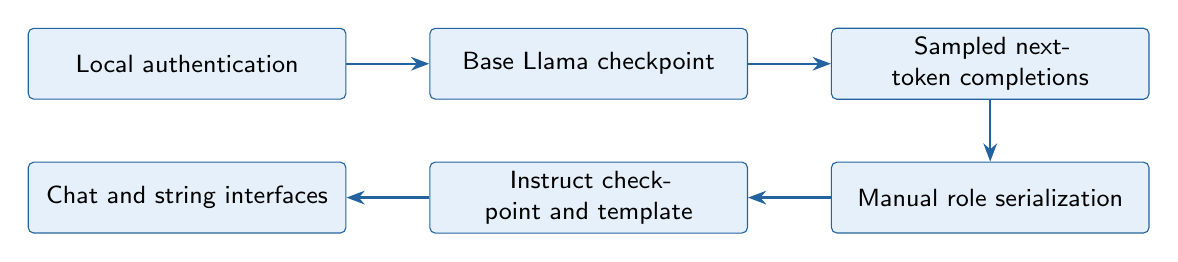
\begin{tikzpicture}[node distance=1cm, >=Stealth,
  stage/.style={draw=steelBlue,fill=skyBlue,rounded corners=2pt,
    align=center,text width=3.8cm,minimum height=0.9cm,font=\small\sffamily}]
\node[stage] (a) at (0cm,0cm) {Local authentication};
\node[stage] (b) at (5.1cm,0cm) {Base Llama checkpoint};
\node[stage] (c) at (10.2cm,0cm) {Sampled next-token completions};
\node[stage] (d) at (10.2cm,-1.7cm) {Manual role serialization};
\node[stage] (e) at (5.1cm,-1.7cm) {Instruct checkpoint and template};
\node[stage] (f) at (0cm,-1.7cm) {Chat and string interfaces};
\draw[->,thick,steelBlue] (a) -- (b);
\draw[->,thick,steelBlue] (b) -- (c);
\draw[->,thick,steelBlue] (c) -- (d);
\draw[->,thick,steelBlue] (d) -- (e);
\draw[->,thick,steelBlue] (e) -- (f);
\end{tikzpicture}%
}
\caption{Exercise pipeline: each stage produces the state consumed by the next.}
\end{figure}

\subsection{Setup and base-model completion}

\medskip
\noindent This setup cell imports the Hub and Transformers APIs, fixes the sampling seed, selects the inference device, and defines a cleanup helper to release a previous model before loading another. The cleanup matters on a memory-limited laptop when the sequence moves from base Llama to instruction-tuned Llama and later to Mistral.
\label{res:lab04-llms-0003}
% coverage-cell: LABS/lab04/text-02-llms.ipynb cell=3 source_sha256=d4b466cc38181a760d8844e3c5f398b1fff4571ebbf142828d9c53d2cc4fc838
\begin{lstlisting}[style=studycode]
from huggingface_hub import login, get_token
import os
import gc

import torch
from transformers import pipeline, AutoTokenizer, AutoModelForCausalLM, set_seed

set_seed(42)
torch.set_num_threads(4)
device = "cuda" if torch.cuda.is_available() else "mps" if torch.backends.mps.is_available() else "cpu"
print(f"Inference backend: {device}")

def release_model():
    # Release the previous pipeline before loading the next multi-billion parameter model.
    globals().pop("pipe", None)
    globals().pop("model", None)
    gc.collect()
    if torch.cuda.is_available():
        torch.cuda.empty_cache()
    elif torch.backends.mps.is_available():
        torch.mps.empty_cache()
\end{lstlisting}
\par\smallskip
% coverage-output: LABS/lab04/text-02-llms.ipynb cell=3 output=0 source_sha256=d4b466cc38181a760d8844e3c5f398b1fff4571ebbf142828d9c53d2cc4fc838 payload_sha256=f43637d18fda73ed60ea94724e2a5c08693605dfc9fe0f578b27b8da90357657 artifact=study_guide/execution_artifacts/lab04/lab04/text-02-llms_cell_0003_d4b466cc3818_output_0.txt
\label{out:lab04-llms-0003-00}
\textit{Complete warning/progress output is retained in the execution-artifact tree and linked to this result.}
% coverage-output: LABS/lab04/text-02-llms.ipynb cell=3 output=1 source_sha256=d4b466cc38181a760d8844e3c5f398b1fff4571ebbf142828d9c53d2cc4fc838 payload_sha256=5eac539957d72a9a57a8e9fb184c65d8d9ae92443e9c8d82f0032532d35c4ffe artifact=study_guide/execution_artifacts/lab04/lab04/text-02-llms_cell_0003_d4b466cc3818_output_1.txt
\label{out:lab04-llms-0003-01}
\lstinputlisting[style=terminalOutput]{../../execution_artifacts/lab04/lab04/text-02-llms_cell_0003_d4b466cc3818_output_1.txt}
The selected backend is MPS. A Jupyter progress-widget warning is retained in the execution artifacts; it does not prevent model loading.

\medskip
\noindent Authentication is read from the user's local Hugging Face credential store. The notebook never embeds a token literal; it passes the local token to the Hub login call with git-credential storage disabled, then deletes the local variable.
\label{res:lab04-llms-0004}
% coverage-cell: LABS/lab04/text-02-llms.ipynb cell=4 source_sha256=819bd4d00231c9f4e92d1b37afc057c1e0cdc5ed8d988d9f5214fc269a6ad8fb
\begin{lstlisting}[style=studycode]
# Login using a local credential; never store the token in the notebook.
token = get_token()
if token is None:
    raise RuntimeError("Llama 3.2 requires an approved Hugging Face account. Run `hf auth login` locally or set HF_TOKEN, then rerun.")
login(token=token, add_to_git_credential=False)
del token
print("Hugging Face authentication configured.")
\end{lstlisting}
\par\smallskip
% coverage-output: LABS/lab04/text-02-llms.ipynb cell=4 output=0 source_sha256=819bd4d00231c9f4e92d1b37afc057c1e0cdc5ed8d988d9f5214fc269a6ad8fb payload_sha256=dd5d2cb7e80c8b7dec73ce0ff626925bdcc43cadfb12ffdb2c858fe6602b9671 artifact=study_guide/execution_artifacts/lab04/lab04/text-02-llms_cell_0004_819bd4d00231_output_0.txt
\label{out:lab04-llms-0004-00}
\lstinputlisting[style=terminalOutput]{../../execution_artifacts/lab04/lab04/text-02-llms_cell_0004_819bd4d00231_output_0.txt}
The cell confirms authentication without printing a credential. Both gated Llama checkpoints were verified accessible for this execution.

\medskip
\noindent This cell loads the base Llama 3.2 1B causal model in FP16, places it on the selected device, switches to evaluation mode, loads its tokenizer, and aliases padding to EOS. The base checkpoint is the next-token-completion model used to establish a non-instruction-tuned baseline.
\label{res:lab04-llms-0008}
% coverage-cell: LABS/lab04/text-02-llms.ipynb cell=8 source_sha256=56c0735d556b32107c6852ec9e1d252e38b4d46fde9a9cb22cc10c649c213e44
\begin{lstlisting}[style=studycode]
model_id = "meta-llama/Llama-3.2-1B"

# TODO: Load the model with `torch.float16` precision and the tokenizer 
# (You can specify the precision with `torch_dtype=torch.float16`)
model = AutoModelForCausalLM.from_pretrained(model_id, torch_dtype=torch.float16, low_cpu_mem_usage=True).to(device).eval()
tokenizer = AutoTokenizer.from_pretrained(model_id)

tokenizer.pad_token = tokenizer.eos_token
\end{lstlisting}
\par\smallskip The model and tokenizer state is ready for five sampled continuations.

\medskip
\noindent The base model generates five continuations from the same short prefix. Sampling draws from the next-token distribution, allowing several plausible continuations; it differs from greedy decoding, which picks one maximum-probability token at each step. Here \texttt{max\_length=50} counts the prompt and continuation together. The returned decoded strings therefore include the prompt and stop near the total-length limit.
\label{res:lab04-llms-0010}
% coverage-cell: LABS/lab04/text-02-llms.ipynb cell=10 source_sha256=0502fff72fa6c134e2a22f8012692617b22d8abe30556e43b2131dbfd2beb6b2
\begin{lstlisting}[style=studycode]
tokens = tokenizer("Hello, my name is", return_tensors="pt").to(model.device)
batch = model.generate(**tokens, do_sample=True, max_length=50, num_return_sequences=5, pad_token_id=tokenizer.eos_token_id) # (assigning pad_token_id avoids a warning)
tokenizer.batch_decode(batch)
\end{lstlisting}
\par\smallskip
% coverage-output: LABS/lab04/text-02-llms.ipynb cell=10 output=0 source_sha256=0502fff72fa6c134e2a22f8012692617b22d8abe30556e43b2131dbfd2beb6b2 payload_sha256=ccfb2c888ce621ae408e8afe38e802779fb56c66ce6f0a0fe1bc9ef50a06b8c0 artifact=study_guide/execution_artifacts/lab04/lab04/text-02-llms_cell_0010_0502fff72fa6_output_0.txt
\label{out:lab04-llms-0010-00}
\lstinputlisting[style=terminalOutput]{../../execution_artifacts/lab04/lab04/text-02-llms_cell_0010_0502fff72fa6_output_0.txt}
The five complete sampled strings show diverse biography-style continuations, including a student, a parent, a dog, and a health-policy worker. They illustrate open-ended completion, not reliable instruction following.

\medskip
\noindent This cell manually defines a Llama 3 conversation serialization: a system header, system content, an end-of-turn token, a user header, and user content. The current date is interpolated at execution. It demonstrates that roles are encoded as control tokens rather than inferred from plain prose.
\label{res:lab04-llms-0012}
% coverage-cell: LABS/lab04/text-02-llms.ipynb cell=12 source_sha256=0d10274c4cdca8af2b670b31655e7b7fa58c06ced63612fa8deb32deb37bdab4
\begin{lstlisting}[style=studycode]
import datetime

chat_template = """
<|begin_of_text|><|start_header_id|>system<|end_header_id|>

Cutting Knowledge Date: December 2023
Today Date: """+datetime.datetime.now().strftime("%d %b %Y")+"""

{system_message}

<|eot_id|>
<|start_header_id|>user<|end_header_id|>

{user_message}

<|eot_id|>
"""
\end{lstlisting}
\par\smallskip The string is a serialization template; this cell has not yet generated an assistant response, and it does not append an explicit assistant-generation prefix.

\medskip
\noindent The text-generation pipeline wraps the already loaded model and tokenizer. It supplies FP16 and the EOS pad ID, then stores the reusable pipeline object for subsequent prompt calls.
\label{res:lab04-llms-0014}
% coverage-cell: LABS/lab04/text-02-llms.ipynb cell=14 source_sha256=ddbdd263da0ce66466f8505965e3b072cf4328961062f3a042c7c455763e9f1c
\begin{lstlisting}[style=studycode]
# Create the pipeline with the model and tokenizer
pipe = pipeline(
    "text-generation",
    model=model,
    tokenizer=tokenizer,
    torch_dtype=torch.float16,
    pad_token_id=tokenizer.eos_token_id,
)
\end{lstlisting}
\par\smallskip
% coverage-output: LABS/lab04/text-02-llms.ipynb cell=14 output=0 source_sha256=ddbdd263da0ce66466f8505965e3b072cf4328961062f3a042c7c455763e9f1c payload_sha256=8892f8f3e6696fc83e83944fce1e482bcb23e747d0b28cfbf91d4b4468b1db6c artifact=study_guide/execution_artifacts/lab04/lab04/text-02-llms_cell_0014_ddbdd263da0c_output_0.txt
\label{out:lab04-llms-0014-00}
\lstinputlisting[style=terminalOutput]{../../execution_artifacts/lab04/lab04/text-02-llms_cell_0014_ddbdd263da0c_output_0.txt}
The saved output warns that no pipeline device was supplied and says the pipeline will use CPU. That warning is important when interpreting these completion timings and outputs: loading the model onto MPS earlier does not make the pipeline's default device choice disappear.

\medskip
\noindent This cell constructs a two-message system/user conversation and manually substitutes their contents into the custom template. Printing the result exposes the exact special-token boundaries before generation. No answer is produced in this cell.
\label{res:lab04-llms-0015}
% coverage-cell: LABS/lab04/text-02-llms.ipynb cell=15 source_sha256=bbe47852e540dac0d2ef1e49d8d88a771033861b316b94863bda105f042c069e
\begin{lstlisting}[style=studycode]

messages = [
    {"role": "system", "content": "You are a pirate chatbot who always responds in pirate speak!"},
    {"role": "user", "content": "What is 2 + 2?"},
]

# Format the messages using the chat template
formatted_messages = chat_template.format(
    system_message=messages[0]["content"],
    user_message=messages[1]["content"]
)


print(formatted_messages)
\end{lstlisting}
\par\smallskip
% coverage-output: LABS/lab04/text-02-llms.ipynb cell=15 output=0 source_sha256=bbe47852e540dac0d2ef1e49d8d88a771033861b316b94863bda105f042c069e payload_sha256=08c96d1e2d3a5a8a10071b9eee2add37093955542f3fc49bceb44e2111869feb artifact=study_guide/execution_artifacts/lab04/lab04/text-02-llms_cell_0015_bbe47852e540_output_0.txt
\label{out:lab04-llms-0015-00}
\lstinputlisting[style=terminalOutput]{../../execution_artifacts/lab04/lab04/text-02-llms_cell_0015_bbe47852e540_output_0.txt}
The output visibly separates the pirate-style system instruction from the arithmetic question with Llama's header and end-of-turn tokens. The next cell sends this complete string to the base model.

\medskip
\noindent The manually serialized string is passed to the base-model pipeline with sampling and a 256-new-token budget. Unlike \texttt{max\_length}, \texttt{max\_new\_tokens} applies only after the prompt. The pipeline returns the full generated text, including the serialized prompt followed by the continuation.
\label{res:lab04-llms-0017}
% coverage-cell: LABS/lab04/text-02-llms.ipynb cell=17 source_sha256=d80dbd1629c28d5e0604989ebe46f45b144e575cc7ecb2d0146d6920d8eb08b2
\begin{lstlisting}[style=studycode]
# Generate the output text 
outputs = pipe(
    formatted_messages,
    max_new_tokens=256,
    do_sample=True,
)

print(outputs[0]["generated_text"])
\end{lstlisting}
\par\smallskip
% coverage-output: LABS/lab04/text-02-llms.ipynb cell=17 output=0 source_sha256=d80dbd1629c28d5e0604989ebe46f45b144e575cc7ecb2d0146d6920d8eb08b2 payload_sha256=a2486fbf39f43b59bdf98a56e87edbb8853f10d834f11d2bb58551a19de205b7 artifact=study_guide/execution_artifacts/lab04/lab04/text-02-llms_cell_0017_d80dbd1629c2_output_0.txt
\label{out:lab04-llms-0017-00}
\lstinputlisting[style=terminalOutput]{../../execution_artifacts/lab04/lab04/text-02-llms_cell_0017_d80dbd1629c2_output_0.txt}
The full output shows how the base completion model continues after the custom conversation serialization. It can imitate the requested style, but the base checkpoint was not trained specifically to obey such instructions.

\subsection{Instruction-tuned model and official chat template}

The role labels are structural metadata once passed as message dictionaries; the Jinja template turns them into the model's learned control-token format. Instruction tuning changes how the checkpoint has been trained to respond to such serialized requests. It is not the same operation as adding role words to a base model's prompt.

\medskip
\noindent The cleanup helper releases the base model before the instruction-tuned checkpoint is loaded. The cell then loads Llama 3.2 1B Instruct, applies the same manually assembled conversation, and uses greedy decoding with up to 512 new tokens. This isolates the checkpoint's instruction-tuning effect while keeping the prompt structure similar.
\label{res:lab04-llms-0019}
% coverage-cell: LABS/lab04/text-02-llms.ipynb cell=19 source_sha256=5fe9a0edd6cf2bc49bf93b380feb4cbd2553c9219b9908b06f4a52e1c3d2d8b0
\begin{lstlisting}[style=studycode]
import torch
from transformers import pipeline, AutoTokenizer, AutoModelForCausalLM

release_model()

model_id = "meta-llama/Llama-3.2-1B-Instruct"

# Load the model with `torch.float16` precision and the tokenizer 
model = AutoModelForCausalLM.from_pretrained(model_id, torch_dtype=torch.float16, low_cpu_mem_usage=True).to(device).eval()
tokenizer = AutoTokenizer.from_pretrained(model_id)

# Set the pad token to the end of the sequence token
tokenizer.pad_token = tokenizer.eos_token

# Create the pipeline with the model and tokenizer
pipe = pipeline(
    "text-generation",
    model=model,
    tokenizer=tokenizer,
    pad_token_id=tokenizer.eos_token_id
)

messages = [
    {"role": "system", "content": "You are a pirate chatbot who always responds in pirate speak!"},
    {"role": "user", "content": "What is 2 + 2?"},
]

# Format the messages using the chat template and generate the output text
formatted_messages = chat_template.format(
    system_message=messages[0]["content"],
    user_message=messages[1]["content"]
)
outputs = pipe(formatted_messages, max_new_tokens=512, do_sample=False)

print(outputs[0]["generated_text"])
\end{lstlisting}
\par\smallskip
% coverage-output: LABS/lab04/text-02-llms.ipynb cell=19 output=0 source_sha256=5fe9a0edd6cf2bc49bf93b380feb4cbd2553c9219b9908b06f4a52e1c3d2d8b0 payload_sha256=8892f8f3e6696fc83e83944fce1e482bcb23e747d0b28cfbf91d4b4468b1db6c artifact=study_guide/execution_artifacts/lab04/lab04/text-02-llms_cell_0019_5fe9a0edd6cf_output_0.txt
\label{out:lab04-llms-0019-00}
\textit{Complete warning/progress output is retained in the execution-artifact tree and linked to this result.}
% coverage-output: LABS/lab04/text-02-llms.ipynb cell=19 output=1 source_sha256=5fe9a0edd6cf2bc49bf93b380feb4cbd2553c9219b9908b06f4a52e1c3d2d8b0 payload_sha256=3a222165572152d2752ac22e7d4d1ed25021182040692157aa935701f3f62fa6 artifact=study_guide/execution_artifacts/lab04/lab04/text-02-llms_cell_0019_5fe9a0edd6cf_output_1.txt
\label{out:lab04-llms-0019-01}
\textit{Complete warning/progress output is retained in the execution-artifact tree and linked to this result.}
% coverage-output: LABS/lab04/text-02-llms.ipynb cell=19 output=2 source_sha256=5fe9a0edd6cf2bc49bf93b380feb4cbd2553c9219b9908b06f4a52e1c3d2d8b0 payload_sha256=d8767dec4b407e2cc466d9ad3e263782bd3aa53213c004bc306f8776af4259c5 artifact=study_guide/execution_artifacts/lab04/lab04/text-02-llms_cell_0019_5fe9a0edd6cf_output_2.txt
\label{out:lab04-llms-0019-02}
\lstinputlisting[style=terminalOutput]{../../execution_artifacts/lab04/lab04/text-02-llms_cell_0019_5fe9a0edd6cf_output_2.txt}
The pipeline and generation configuration warnings are retained in the execution artifacts. The actual generated string follows the pirate persona and answers the arithmetic question. Greedy decoding is deterministic for a fixed model, prompt, and implementation, but it does not guarantee correctness in general.

\medskip
\noindent This cell prints the instruction tokenizer's complete Jinja chat template. The template encodes role headers, tool branches, message endings, and an optional assistant-generation prefix. Reading the actual template clarifies why a list of role dictionaries is not equivalent to concatenating labels into ordinary text.
\label{res:lab04-llms-0021}
% coverage-cell: LABS/lab04/text-02-llms.ipynb cell=21 source_sha256=9f6e6aee8660c79b3b89251cce515c0d2d7b8177f57c66560a03a076c792db21
\begin{lstlisting}[style=studycode]
model_id = "meta-llama/Llama-3.2-1B-Instruct"

tokenizer = AutoTokenizer.from_pretrained(model_id)

print(tokenizer.chat_template)
\end{lstlisting}
\par\smallskip
% coverage-output: LABS/lab04/text-02-llms.ipynb cell=21 output=0 source_sha256=9f6e6aee8660c79b3b89251cce515c0d2d7b8177f57c66560a03a076c792db21 payload_sha256=2f464620485f0f81f404553366d995c7478029feed8e0b34289d58a16699dd96 artifact=study_guide/execution_artifacts/lab04/lab04/text-02-llms_cell_0021_9f6e6aee8660_output_0.txt
\label{out:lab04-llms-0021-00}
\lstinputlisting[style=terminalOutput]{../../execution_artifacts/lab04/lab04/text-02-llms_cell_0021_9f6e6aee8660_output_0.txt}
The complete printed template is reproduced. Its conditional branches serialize messages according to role and control tokens; later calls use \texttt{apply\_chat\_template} so these boundaries are supplied by the tokenizer's official template.

\medskip
\noindent This cell creates a text-generation pipeline and passes the conversation as a list of role dictionaries. It separately prints the result of applying the chat template with \texttt{add\_generation\_prompt=True}, then calls the pipeline in chat mode and selects the last assistant message's content.
\label{res:lab04-llms-0024}
% coverage-cell: LABS/lab04/text-02-llms.ipynb cell=24 source_sha256=9c3416c7a2679742e2a3fe5e80efcd31fa8482fdbf0201aa486fb118bcd80a54
\begin{lstlisting}[style=studycode]
# TODO: Create the pipeline with the model and tokenizer
pipe = pipeline("text-generation", model=model, tokenizer=tokenizer, pad_token_id=tokenizer.eos_token_id)

messages = [
    {"role": "system", "content": "You are a pirate chatbot who always responds in pirate speak!"},
    {"role": "user", "content": "Who are you?"},
]
input_tokens = tokenizer.apply_chat_template(messages, add_generation_prompt=True)
print(tokenizer.decode(input_tokens))

# Generate in pipeline chat mode; it applies the same chat template internally.
outputs = pipe(messages, max_new_tokens=100, do_sample=False)

# we are getting back the full conversation history
# as a list of messages outputs[0]["generated_text"]
# -1 : last message (assistant response)
print(outputs[0]["generated_text"][-1]["content"])
\end{lstlisting}
\par\smallskip
% coverage-output: LABS/lab04/text-02-llms.ipynb cell=24 output=0 source_sha256=9c3416c7a2679742e2a3fe5e80efcd31fa8482fdbf0201aa486fb118bcd80a54 payload_sha256=8892f8f3e6696fc83e83944fce1e482bcb23e747d0b28cfbf91d4b4468b1db6c artifact=study_guide/execution_artifacts/lab04/lab04/text-02-llms_cell_0024_9c3416c7a267_output_0.txt
\label{out:lab04-llms-0024-00}
\textit{Complete warning/progress output is retained in the execution-artifact tree and linked to this result.}
% coverage-output: LABS/lab04/text-02-llms.ipynb cell=24 output=1 source_sha256=9c3416c7a2679742e2a3fe5e80efcd31fa8482fdbf0201aa486fb118bcd80a54 payload_sha256=f72780f41b0b366fc4ef9bffd5fb0ae07741f903a973cf11c3fd452b9cf5c39a artifact=study_guide/execution_artifacts/lab04/lab04/text-02-llms_cell_0024_9c3416c7a267_output_1.txt
\label{out:lab04-llms-0024-01}
\lstinputlisting[style=terminalOutput]{../../execution_artifacts/lab04/lab04/text-02-llms_cell_0024_9c3416c7a267_output_1.txt}
% coverage-output: LABS/lab04/text-02-llms.ipynb cell=24 output=2 source_sha256=9c3416c7a2679742e2a3fe5e80efcd31fa8482fdbf0201aa486fb118bcd80a54 payload_sha256=ad207700120fc6c6314211e5cc0163f228e5cc0434b20d273b55ef1a5d985c11 artifact=study_guide/execution_artifacts/lab04/lab04/text-02-llms_cell_0024_9c3416c7a267_output_2.txt
\label{out:lab04-llms-0024-02}
\lstinputlisting[style=terminalOutput]{../../execution_artifacts/lab04/lab04/text-02-llms_cell_0024_9c3416c7a267_output_2.txt}
The first output shows the serialized prompt ending at an assistant-generation prefix; the second is only the assistant's pirate-style response. The pipeline accepts chat messages and returns the full conversation as a list of messages, from which this code extracts the last one. A CPU-default warning is preserved in the execution artifacts.

\medskip
\noindent This cell applies the same official template manually, decodes the token IDs while retaining special tokens, and passes the result as a string. \texttt{add\_special\_tokens=False} is essential: the string already contains its BOS and role-control tokens, so adding another BOS would duplicate serialization markers.
\label{res:lab04-llms-0026}
% coverage-cell: LABS/lab04/text-02-llms.ipynb cell=26 source_sha256=5fc77adf50bf2b98fe6df6ec6a476ca779a47b1ca83e8be60aaac069b339e4f5
\begin{lstlisting}[style=studycode]
messages = [
    {"role": "system", "content": "You are a pirate chatbot who always responds in pirate speak!"},
    {"role": "user", "content": "Who are you?"},
]

# TODO: Format the messages using the chat template and generate the output text
input_tokens = tokenizer.apply_chat_template(messages, add_generation_prompt=True)
prompt_string = tokenizer.decode(input_tokens, skip_special_tokens=False)

outputs = pipe(prompt_string, max_new_tokens=100, do_sample=False, add_special_tokens=False)

print(outputs[0]["generated_text"])
\end{lstlisting}
\par\smallskip
% coverage-output: LABS/lab04/text-02-llms.ipynb cell=26 output=0 source_sha256=5fc77adf50bf2b98fe6df6ec6a476ca779a47b1ca83e8be60aaac069b339e4f5 payload_sha256=889955e64cb49fc05b3f4d023e47df4ad4df77adf9016d18692b6791f9c4f2b3 artifact=study_guide/execution_artifacts/lab04/lab04/text-02-llms_cell_0026_5fc77adf50bf_output_0.txt
\label{out:lab04-llms-0026-00}
\lstinputlisting[style=terminalOutput]{../../execution_artifacts/lab04/lab04/text-02-llms_cell_0026_5fc77adf50bf_output_0.txt}
The string-mode output contains both the serialized prompt and generated response. This return shape differs from chat mode: chat mode returns a message list, while string mode returns one combined text string.

\begin{quote}\noindent\textbf{A chat template is a serializer.} 

A chat template is a serializer: it maps a list such as system/user messages into a sequence containing role headers, content, and end markers. The instruction-tuned weights supply the learned behavior associated with those sequences. A serializer alone does not instruction-tune a base checkpoint.

\end{quote}

\clearpage

\section{Exercise 3: Mistral structured answers}

\label{sec:lab04-mistral}

The final exercise uses Mistral 7B Instruct v0.2 with Quanto INT4 weights on the 16 GiB MPS machine. It first demonstrates a role-conditioned response, then generates five seeded addition questions under a JSON-only system instruction. The saved conversations retain trusted operands so the verifier can check JSON syntax, operand identity, and arithmetic separately; malformed or incomplete answers must fail those checks.

\begin{figure}[htbp]
\centering
\resizebox{\linewidth}{!}{%
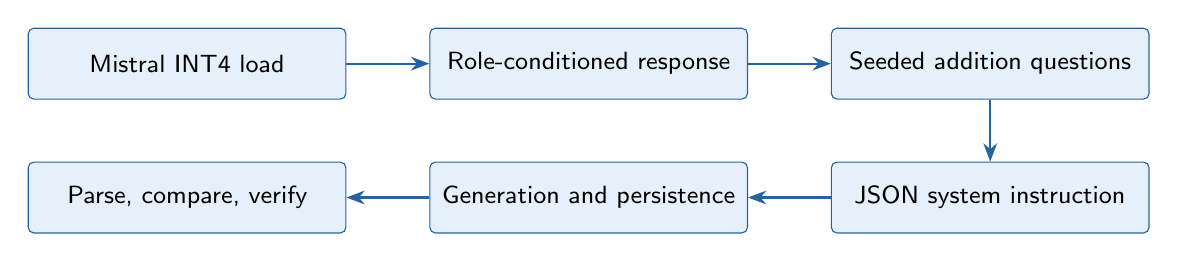
\begin{tikzpicture}[node distance=1cm, >=Stealth,
  stage/.style={draw=steelBlue,fill=skyBlue,rounded corners=2pt,
    align=center,text width=3.8cm,minimum height=0.9cm,font=\small\sffamily}]
\node[stage] (a) at (0cm,0cm) {Mistral INT4 load};
\node[stage] (b) at (5.1cm,0cm) {Role-conditioned response};
\node[stage] (c) at (10.2cm,0cm) {Seeded addition questions};
\node[stage] (d) at (10.2cm,-1.7cm) {JSON system instruction};
\node[stage] (e) at (5.1cm,-1.7cm) {Generation and persistence};
\node[stage] (f) at (0cm,-1.7cm) {Parse, compare, verify};
\draw[->,thick,steelBlue] (a) -- (b);
\draw[->,thick,steelBlue] (b) -- (c);
\draw[->,thick,steelBlue] (c) -- (d);
\draw[->,thick,steelBlue] (d) -- (e);
\draw[->,thick,steelBlue] (e) -- (f);
\end{tikzpicture}%
}
\caption{Exercise pipeline: each stage produces the state consumed by the next.}
\end{figure}

\subsection{Model setup and role-conditioned response}

\medskip
\noindent The Mistral cell releases the prior model, loads Mistral 7B Instruct v0.2, and chooses Quanto INT4 weights on this MPS machine with less than 24 GiB of physical memory; larger machines retain FP16. It then sets EOS as padding, builds a text-generation pipeline, and sends a system/user message list. This is a role-conditioned inference example, separate from the later structured-output task.
\label{res:lab04-llms-0029}
% coverage-cell: LABS/lab04/text-02-llms.ipynb cell=29 source_sha256=9b1a4f06ae574ddcfaf74e4ebc1d4f1aff3389b900c8ee377d109699e810171a
\begin{lstlisting}[style=studycode]
# Define the model ID
release_model()

model_id = "mistralai/Mistral-7B-Instruct-v0.2"

# TODO: Load the model and the tokenizer 
# The 7B FP16 weights alone take about 14.5 GB. On this 16 GB Mac,
# load the same checkpoint with 4-bit weights; retain FP16 on larger machines.
from transformers import QuantoConfig
import psutil
use_int4 = device == "mps" and psutil.virtual_memory().total < 24 * 1024**3
load_options = {"quantization_config": QuantoConfig(weights="int4")} if use_int4 else {}
model = AutoModelForCausalLM.from_pretrained(
    model_id, torch_dtype=torch.float16, device_map=device,
    low_cpu_mem_usage=True, **load_options,
).eval()
print("Mistral weights:", "int4 (Quanto)" if use_int4 else "float16")

tokenizer = AutoTokenizer.from_pretrained(model_id)
tokenizer.pad_token = tokenizer.eos_token

# TODO: Initialize the pipeline for text generation
pipe = pipeline("text-generation", model=model, tokenizer=tokenizer, pad_token_id=tokenizer.eos_token_id)

# Define the message prompts for the conversation
messages = [
    {"role": "system", "content": "You are a pirate chatbot who always responds in pirate speak!"},
    {"role": "user", "content": "Who are you?"}
]

# TODO: Generate the response
outputs = pipe(messages, max_new_tokens=100, pad_token_id=tokenizer.eos_token_id)

# Print the model's generated response
print(outputs[0]["generated_text"][-1]["content"])
\end{lstlisting}
\par\smallskip
% coverage-output: LABS/lab04/text-02-llms.ipynb cell=29 output=0 source_sha256=9b1a4f06ae574ddcfaf74e4ebc1d4f1aff3389b900c8ee377d109699e810171a payload_sha256=6c56fe5790369a690a1488c6e2f711f3440f61daa3969824a64809236ee828db artifact=study_guide/execution_artifacts/lab04/lab04/text-02-llms_cell_0029_9b1a4f06ae57_output_0.txt
\label{out:lab04-llms-0029-00}
\textit{Complete warning/progress output is retained in the execution-artifact tree and linked to this result.}
% coverage-output: LABS/lab04/text-02-llms.ipynb cell=29 output=1 source_sha256=9b1a4f06ae574ddcfaf74e4ebc1d4f1aff3389b900c8ee377d109699e810171a payload_sha256=119b4738ff55eb4173655bce31e1398f931aa5f608712dc61f06563353a9fe4f artifact=study_guide/execution_artifacts/lab04/lab04/text-02-llms_cell_0029_9b1a4f06ae57_output_1.txt
\label{out:lab04-llms-0029-01}
\textit{Complete warning/progress output is retained in the execution-artifact tree and linked to this result.}
% coverage-output: LABS/lab04/text-02-llms.ipynb cell=29 output=2 source_sha256=9b1a4f06ae574ddcfaf74e4ebc1d4f1aff3389b900c8ee377d109699e810171a payload_sha256=de359ccfc6372fc924925bcea9b927b6b3334165c06f702cc0b8b70c190a4162 artifact=study_guide/execution_artifacts/lab04/lab04/text-02-llms_cell_0029_9b1a4f06ae57_output_2.txt
\label{out:lab04-llms-0029-02}
\textit{Complete warning/progress output is retained in the execution-artifact tree and linked to this result.}
% coverage-output: LABS/lab04/text-02-llms.ipynb cell=29 output=3 source_sha256=9b1a4f06ae574ddcfaf74e4ebc1d4f1aff3389b900c8ee377d109699e810171a payload_sha256=77d5ab44d5fa9b84caea7e8d1b35ac37c2d1aa0d769ed690ce2891a921f30b93 artifact=study_guide/execution_artifacts/lab04/lab04/text-02-llms_cell_0029_9b1a4f06ae57_output_3.txt
\label{out:lab04-llms-0029-03}
\textit{Complete warning/progress output is retained in the execution-artifact tree and linked to this result.}
% coverage-output: LABS/lab04/text-02-llms.ipynb cell=29 output=4 source_sha256=9b1a4f06ae574ddcfaf74e4ebc1d4f1aff3389b900c8ee377d109699e810171a payload_sha256=21f82e3e1cda217ad9d8746e0da74811f0c9702b73fc834f2f25254d043cad5f artifact=study_guide/execution_artifacts/lab04/lab04/text-02-llms_cell_0029_9b1a4f06ae57_output_4.txt
\label{out:lab04-llms-0029-04}
\textit{Complete warning/progress output is retained in the execution-artifact tree and linked to this result.}
% coverage-output: LABS/lab04/text-02-llms.ipynb cell=29 output=5 source_sha256=9b1a4f06ae574ddcfaf74e4ebc1d4f1aff3389b900c8ee377d109699e810171a payload_sha256=20edaa3e50bf40ea9d7f0ac1fb0c44b3e7771949761d7a46df51f9ab1ceac876 artifact=-
\label{out:lab04-llms-0029-05}
\textit{Complete warning/progress output is retained in the execution-artifact tree and linked to this result.}
% coverage-output: LABS/lab04/text-02-llms.ipynb cell=29 output=6 source_sha256=9b1a4f06ae574ddcfaf74e4ebc1d4f1aff3389b900c8ee377d109699e810171a payload_sha256=7d144d4e0aa0a6312e148f98abdfb2fc13d902e2701f39fdbdd47352017b404d artifact=study_guide/execution_artifacts/lab04/lab04/text-02-llms_cell_0029_9b1a4f06ae57_output_6.txt
\label{out:lab04-llms-0029-06}
\textit{Complete warning/progress output is retained in the execution-artifact tree and linked to this result.}
% coverage-output: LABS/lab04/text-02-llms.ipynb cell=29 output=7 source_sha256=9b1a4f06ae574ddcfaf74e4ebc1d4f1aff3389b900c8ee377d109699e810171a payload_sha256=e102033e7b0b0b809d63014e7f65b4ccc2b79d507675c298f0fc6515a5af2632 artifact=study_guide/execution_artifacts/lab04/lab04/text-02-llms_cell_0029_9b1a4f06ae57_output_7.txt
\label{out:lab04-llms-0029-07}
\textit{Complete warning/progress output is retained in the execution-artifact tree and linked to this result.}
% coverage-output: LABS/lab04/text-02-llms.ipynb cell=29 output=8 source_sha256=9b1a4f06ae574ddcfaf74e4ebc1d4f1aff3389b900c8ee377d109699e810171a payload_sha256=cd205113b2cc40b09983087b924f71a6b98320b4e9597ba799facf67eb379fdb artifact=study_guide/execution_artifacts/lab04/lab04/text-02-llms_cell_0029_9b1a4f06ae57_output_8.txt
\label{out:lab04-llms-0029-08}
\textit{Complete warning/progress output is retained in the execution-artifact tree and linked to this result.}
% coverage-output: LABS/lab04/text-02-llms.ipynb cell=29 output=9 source_sha256=9b1a4f06ae574ddcfaf74e4ebc1d4f1aff3389b900c8ee377d109699e810171a payload_sha256=d485e4f1019efb0c217a2ae9edbfaa42f4110b30795bc8e3e8c34e5ccd04d3f1 artifact=study_guide/execution_artifacts/lab04/lab04/text-02-llms_cell_0029_9b1a4f06ae57_output_9.txt
\label{out:lab04-llms-0029-09}
\lstinputlisting[style=terminalOutput]{../../execution_artifacts/lab04/lab04/text-02-llms_cell_0029_9b1a4f06ae57_output_9.txt}
The run reports Quanto INT4 weights and a pirate-style self-description. Loading progress and tokenizer fork warnings are retained in the execution artifacts. The role-conditioned answer demonstrates format and persona behavior only.

\subsection{Question generation and JSON instruction}

\medskip
\noindent This cell seeds Python's random generator and defines five natural-language templates for addition questions. Each generated record includes the rendered question and both integer operands, so verification can compare the model's parsed operands as well as its sum.
\label{res:lab04-llms-0032}
% coverage-cell: LABS/lab04/text-02-llms.ipynb cell=32 source_sha256=04942a2b7a11ed4c11893bc01c27d0e471ff1de605d7e3b2da178fedd494459f
\begin{lstlisting}[style=studycode]
import random
random.seed(42)

def generate_random_math_questions(num_samples=5):
    """
    Generate random math questions with two numbers for a given number of samples.

    Args:
        num_samples (int): The number of math questions to generate.
    
    Returns:
        List of tuples: A list of tuples containing the math question and the two numbers (question, num1, num2).
    """

    # Define templates for math questions with two numbers
    templates = [
        "What is the sum of {} and {}?",
        "Can you add {} and {}?",
        "Calculate the sum of {} and {} for me.",
        "How much is {} plus {}?",
        "Please add {} and {}."
    ]
    
    questions = []
    for _ in range(num_samples):
        # TODO: Randomly select a template and generate two random numbers
        template = random.choice(templates)
        num1 = random.randint(1, 1000)
        num2 = random.randint(1, 1000)
        question = template.format(num1, num2)
        questions.append((question, num1, num2))  # store question with numbers for validation
    return questions
\end{lstlisting}
\par\smallskip This function prepares five sampled questions for the following generation cell.

\medskip
\noindent This cell defines the system instruction for structured answering. It requires JSON with \texttt{num\_1}, \texttt{num\_2}, and \texttt{answer}, and asks the model to emit only JSON so a parser can consume it.
\label{res:lab04-llms-0034}
% coverage-cell: LABS/lab04/text-02-llms.ipynb cell=34 source_sha256=aafc2120e867513a8447451d8880dcbeb4a3b3f6a3754299ae8dfceb5449d927
\begin{lstlisting}[style=studycode]
role_instruction = {
    "role": "system",
    "content": "Answer each question in JSON format with the fields 'num_1', 'num_2', and 'answer'. Provide only JSON to ensure compatibility with a JSON parser."
}
\end{lstlisting}
\par\smallskip The role dictionary is prepended to every user question by the next cell.

\subsection{Generate, save, parse, and verify}

\medskip
\noindent This cell generates five seeded addition questions, sends each as a system/user chat, and stores the pipeline's full generated message list alongside the trusted operands. It then persists the records as \texttt{model\_answers.json}. The progress bar is diagnostic output; the saved file is the durable result used by verification.
\label{res:lab04-llms-0036}
% coverage-cell: LABS/lab04/text-02-llms.ipynb cell=36 source_sha256=49b817fbd01221bacb802b6777eba8e5a87d3b3a64cf09227c92107ae57ca478
\begin{lstlisting}[style=studycode]
import json
from tqdm import tqdm

# Generate questions and answers, then save to JSON
questions = generate_random_math_questions(num_samples=5)
answers = []

# Generate structured answers for each question
for question, num1, num2 in tqdm(questions):
    # TODO: Define the message prompts
    formatted_messages = [role_instruction, {"role": "user", "content": question}]
    
    # TODO: Generate the response
    outputs = pipe(formatted_messages, max_new_tokens=100, do_sample=False, pad_token_id=tokenizer.eos_token_id)
    
    # Extract the model's JSON output
    structured_answer = outputs[0]["generated_text"]

    answers.append({
        "question": question,
        "num_1": num1,
        "num_2": num2,
        "model_answer": structured_answer
    })

# Save answers to a JSON file
with open("model_answers.json", "w") as f:
    json.dump(answers, f, indent=2)
\end{lstlisting}
\par\smallskip
% coverage-output: LABS/lab04/text-02-llms.ipynb cell=36 output=0 source_sha256=49b817fbd01221bacb802b6777eba8e5a87d3b3a64cf09227c92107ae57ca478 payload_sha256=4148e90b82c1ade033fa4add138e7b5adf530423d0d27e8edc85cd5cbc7a94e1 artifact=study_guide/execution_artifacts/lab04/lab04/text-02-llms_cell_0036_49b817fbd012_output_0.txt
\label{out:lab04-llms-0036-00}
\textit{Complete warning/progress output is retained in the execution-artifact tree and linked to this result.}
% coverage-output: LABS/lab04/text-02-llms.ipynb cell=36 output=1 source_sha256=49b817fbd01221bacb802b6777eba8e5a87d3b3a64cf09227c92107ae57ca478 payload_sha256=62a067979d0ce165a1a46b7a6a5ad9b3da7da146d6a8ff22340f0bb7ade1aa93 artifact=study_guide/execution_artifacts/lab04/lab04/text-02-llms_cell_0036_49b817fbd012_output_1.txt
\label{out:lab04-llms-0036-01}
\textit{Complete warning/progress output is retained in the execution-artifact tree and linked to this result.}
% coverage-output: LABS/lab04/text-02-llms.ipynb cell=36 output=2 source_sha256=49b817fbd01221bacb802b6777eba8e5a87d3b3a64cf09227c92107ae57ca478 payload_sha256=a83a68642f80d196afb95efd6a55971bf32331667bbd5e666995777cddde3841 artifact=study_guide/execution_artifacts/lab04/lab04/text-02-llms_cell_0036_49b817fbd012_output_2.txt
\label{out:lab04-llms-0036-02}
\textit{Complete warning/progress output is retained in the execution-artifact tree and linked to this result.}
% coverage-output: LABS/lab04/text-02-llms.ipynb cell=36 output=3 source_sha256=49b817fbd01221bacb802b6777eba8e5a87d3b3a64cf09227c92107ae57ca478 payload_sha256=911294955ea1eb0e5da8dc9b41d7e98e378e8ca79576f7bacd484ea8498284d9 artifact=study_guide/execution_artifacts/lab04/lab04/text-02-llms_cell_0036_49b817fbd012_output_3.txt
\label{out:lab04-llms-0036-03}
\textit{Complete warning/progress output is retained in the execution-artifact tree and linked to this result.}
% coverage-output: LABS/lab04/text-02-llms.ipynb cell=36 output=4 source_sha256=49b817fbd01221bacb802b6777eba8e5a87d3b3a64cf09227c92107ae57ca478 payload_sha256=dcadcfc994f9e90d5b2c6c08ceb4d18c6f16f690f378daa73d5ff3bfbc43c86f artifact=study_guide/execution_artifacts/lab04/lab04/text-02-llms_cell_0036_49b817fbd012_output_4.txt
\label{out:lab04-llms-0036-04}
\textit{Complete warning/progress output is retained in the execution-artifact tree and linked to this result.}
% coverage-output: LABS/lab04/text-02-llms.ipynb cell=36 output=5 source_sha256=49b817fbd01221bacb802b6777eba8e5a87d3b3a64cf09227c92107ae57ca478 payload_sha256=116a8618063eb05d178f2272c2200901ff2ba3000e8bd26f7481ec857dca3643 artifact=study_guide/execution_artifacts/lab04/lab04/text-02-llms_cell_0036_49b817fbd012_output_5.txt
\label{out:lab04-llms-0036-05}
\textit{Complete warning/progress output is retained in the execution-artifact tree and linked to this result.}
% coverage-output: LABS/lab04/text-02-llms.ipynb cell=36 output=6 source_sha256=49b817fbd01221bacb802b6777eba8e5a87d3b3a64cf09227c92107ae57ca478 payload_sha256=5a9d3a09ce3a35da5ec3b0550bbddfefb711969562c5678d944b71d5de330291 artifact=study_guide/execution_artifacts/lab04/lab04/text-02-llms_cell_0036_49b817fbd012_output_6.txt
\label{out:lab04-llms-0036-06}
\textit{Complete warning/progress output is retained in the execution-artifact tree and linked to this result.}
% coverage-output: LABS/lab04/text-02-llms.ipynb cell=36 output=7 source_sha256=49b817fbd01221bacb802b6777eba8e5a87d3b3a64cf09227c92107ae57ca478 payload_sha256=20edaa3e50bf40ea9d7f0ac1fb0c44b3e7771949761d7a46df51f9ab1ceac876 artifact=-
\label{out:lab04-llms-0036-07}
\textit{This notebook output slot contains no printable text representation.}
The cell creates five answer records. The exact saved JSON is included after this code, preserving both the assistant messages and the expected operands. Its progress trace is retained in the execution artifacts.

\paragraph{Saved side-effect artifact.} The loop writes the following complete file. The \texttt{model\_answer} value preserves the full system/user/assistant message list, while the outer operands remain the verification reference.

% coverage-artifact: LABS/lab04/text-02-llms.ipynb::cell-0036 source_sha256=49b817fbd01221bacb802b6777eba8e5a87d3b3a64cf09227c92107ae57ca478 path=lab04/model_answers.json sha256=ba4794797d373dfd9a4e67195781a02abad66e6c34751146fd2969cf2254db49

\label{out:lab04-mistral-json-file}

\lstinputlisting[style=terminalOutput]{../../../lab04/model_answers.json}

\medskip
\noindent The verification function locates the assistant message, parses its content with \texttt{json.loads}, checks that both parsed operands match the original question, and only then checks that the answer equals their sum. Missing messages, malformed JSON, missing fields, and type/value errors are caught and rejected.
\label{res:lab04-llms-0037}
% coverage-cell: LABS/lab04/text-02-llms.ipynb cell=37 source_sha256=bbb6347798f4da8605fe94947ca94e99acb6dbbd9f3de5acaae01d68b4a670e6
\begin{lstlisting}[style=studycode]
import json

# Function to parse model's answer and verify correctness
def verify_answer(entry):
    try:
        # Extract expected values
        num1, num2 = entry["num_1"], entry["num_2"]
        expected_answer = num1 + num2
        
        # Extract the assistant's response from the list of messages
        assistant_message = next(
            (msg["content"] for msg in entry["model_answer"] if msg["role"] == "assistant"), None
        )
        
        if assistant_message is None:
            raise ValueError("Assistant's message not found in model_answer")
        
        # Parse model's structured answer from JSON
        model_response = json.loads(assistant_message.strip())  # Ensure model_answer is a string
        
        print(f"Expected answer: {num1} + {num2} = {expected_answer}")
        print(f"Model's answer: {model_response['num_1']} + {model_response['num_2']} = {model_response['answer']}")
        
        # Check if the values match
        if (model_response["num_1"] == num1 and 
            model_response["num_2"] == num2 and 
            model_response["answer"] == expected_answer):
            return True
        else:
            return False
    except (json.JSONDecodeError, KeyError, TypeError, ValueError) as e:
        # Handle cases where parsing fails or keys are missing
        print(f"Error verifying entry: {entry}. Error: {e}")
        return False

# Load answers from the JSON file and verify
try:
    with open("model_answers.json", "r") as f:
        saved_answers = json.load(f)
except (json.JSONDecodeError, FileNotFoundError) as e:
    print(f"Error loading JSON file: {e}")
    saved_answers = []

for i, entry in enumerate(saved_answers, 1):
    result = verify_answer(entry)
    print(f"Question {i}:", "Correct" if result else "Incorrect", "\n")
\end{lstlisting}
\par\smallskip
% coverage-output: LABS/lab04/text-02-llms.ipynb cell=37 output=0 source_sha256=bbb6347798f4da8605fe94947ca94e99acb6dbbd9f3de5acaae01d68b4a670e6 payload_sha256=f92bcbd6ac075984a3be7e09308ab0a6eebcb38957cc43e99b839dad6c3864cb artifact=study_guide/execution_artifacts/lab04/lab04/text-02-llms_cell_0037_bbb6347798f4_output_0.txt
\label{out:lab04-llms-0037-00}
\lstinputlisting[style=terminalOutput]{../../execution_artifacts/lab04/lab04/text-02-llms_cell_0037_bbb6347798f4_output_0.txt}
All five saved examples pass: each response is valid JSON, repeats the correct operands, and gives the correct sum. Additional negative-case checks reject a missing assistant message, malformed JSON, a missing field, and an incorrect answer. Five correct samples do not establish general arithmetic reliability.

\begin{center}

\begin{tabularx}{\linewidth}{l r r r X}

\toprule

Case & JSON parses & Operands match & Sum correct & Verification result\\

\midrule

Five saved records & Yes & Yes & Yes & Accepted in the notebook output\\

Assistant message missing & -- & -- & -- & Rejected with a value error\\

Malformed JSON & No & -- & -- & Rejected by the JSON parser\\

Required field missing & Yes & -- & -- & Rejected by key lookup\\

Wrong arithmetic result & Yes & Yes & No & Returned as incorrect\\

\bottomrule

\end{tabularx}

\end{center}

The acceptance table separates three checks that are often conflated. Syntactically valid JSON can still contain wrong operands or an incorrect answer. The five successes validate these five examples only; they do not establish general arithmetic reliability.

\end{document}

\end{document}
